
\section{RoboGuard}
\label{sec:method}

\begin{figure}[ht!]
    \centering
    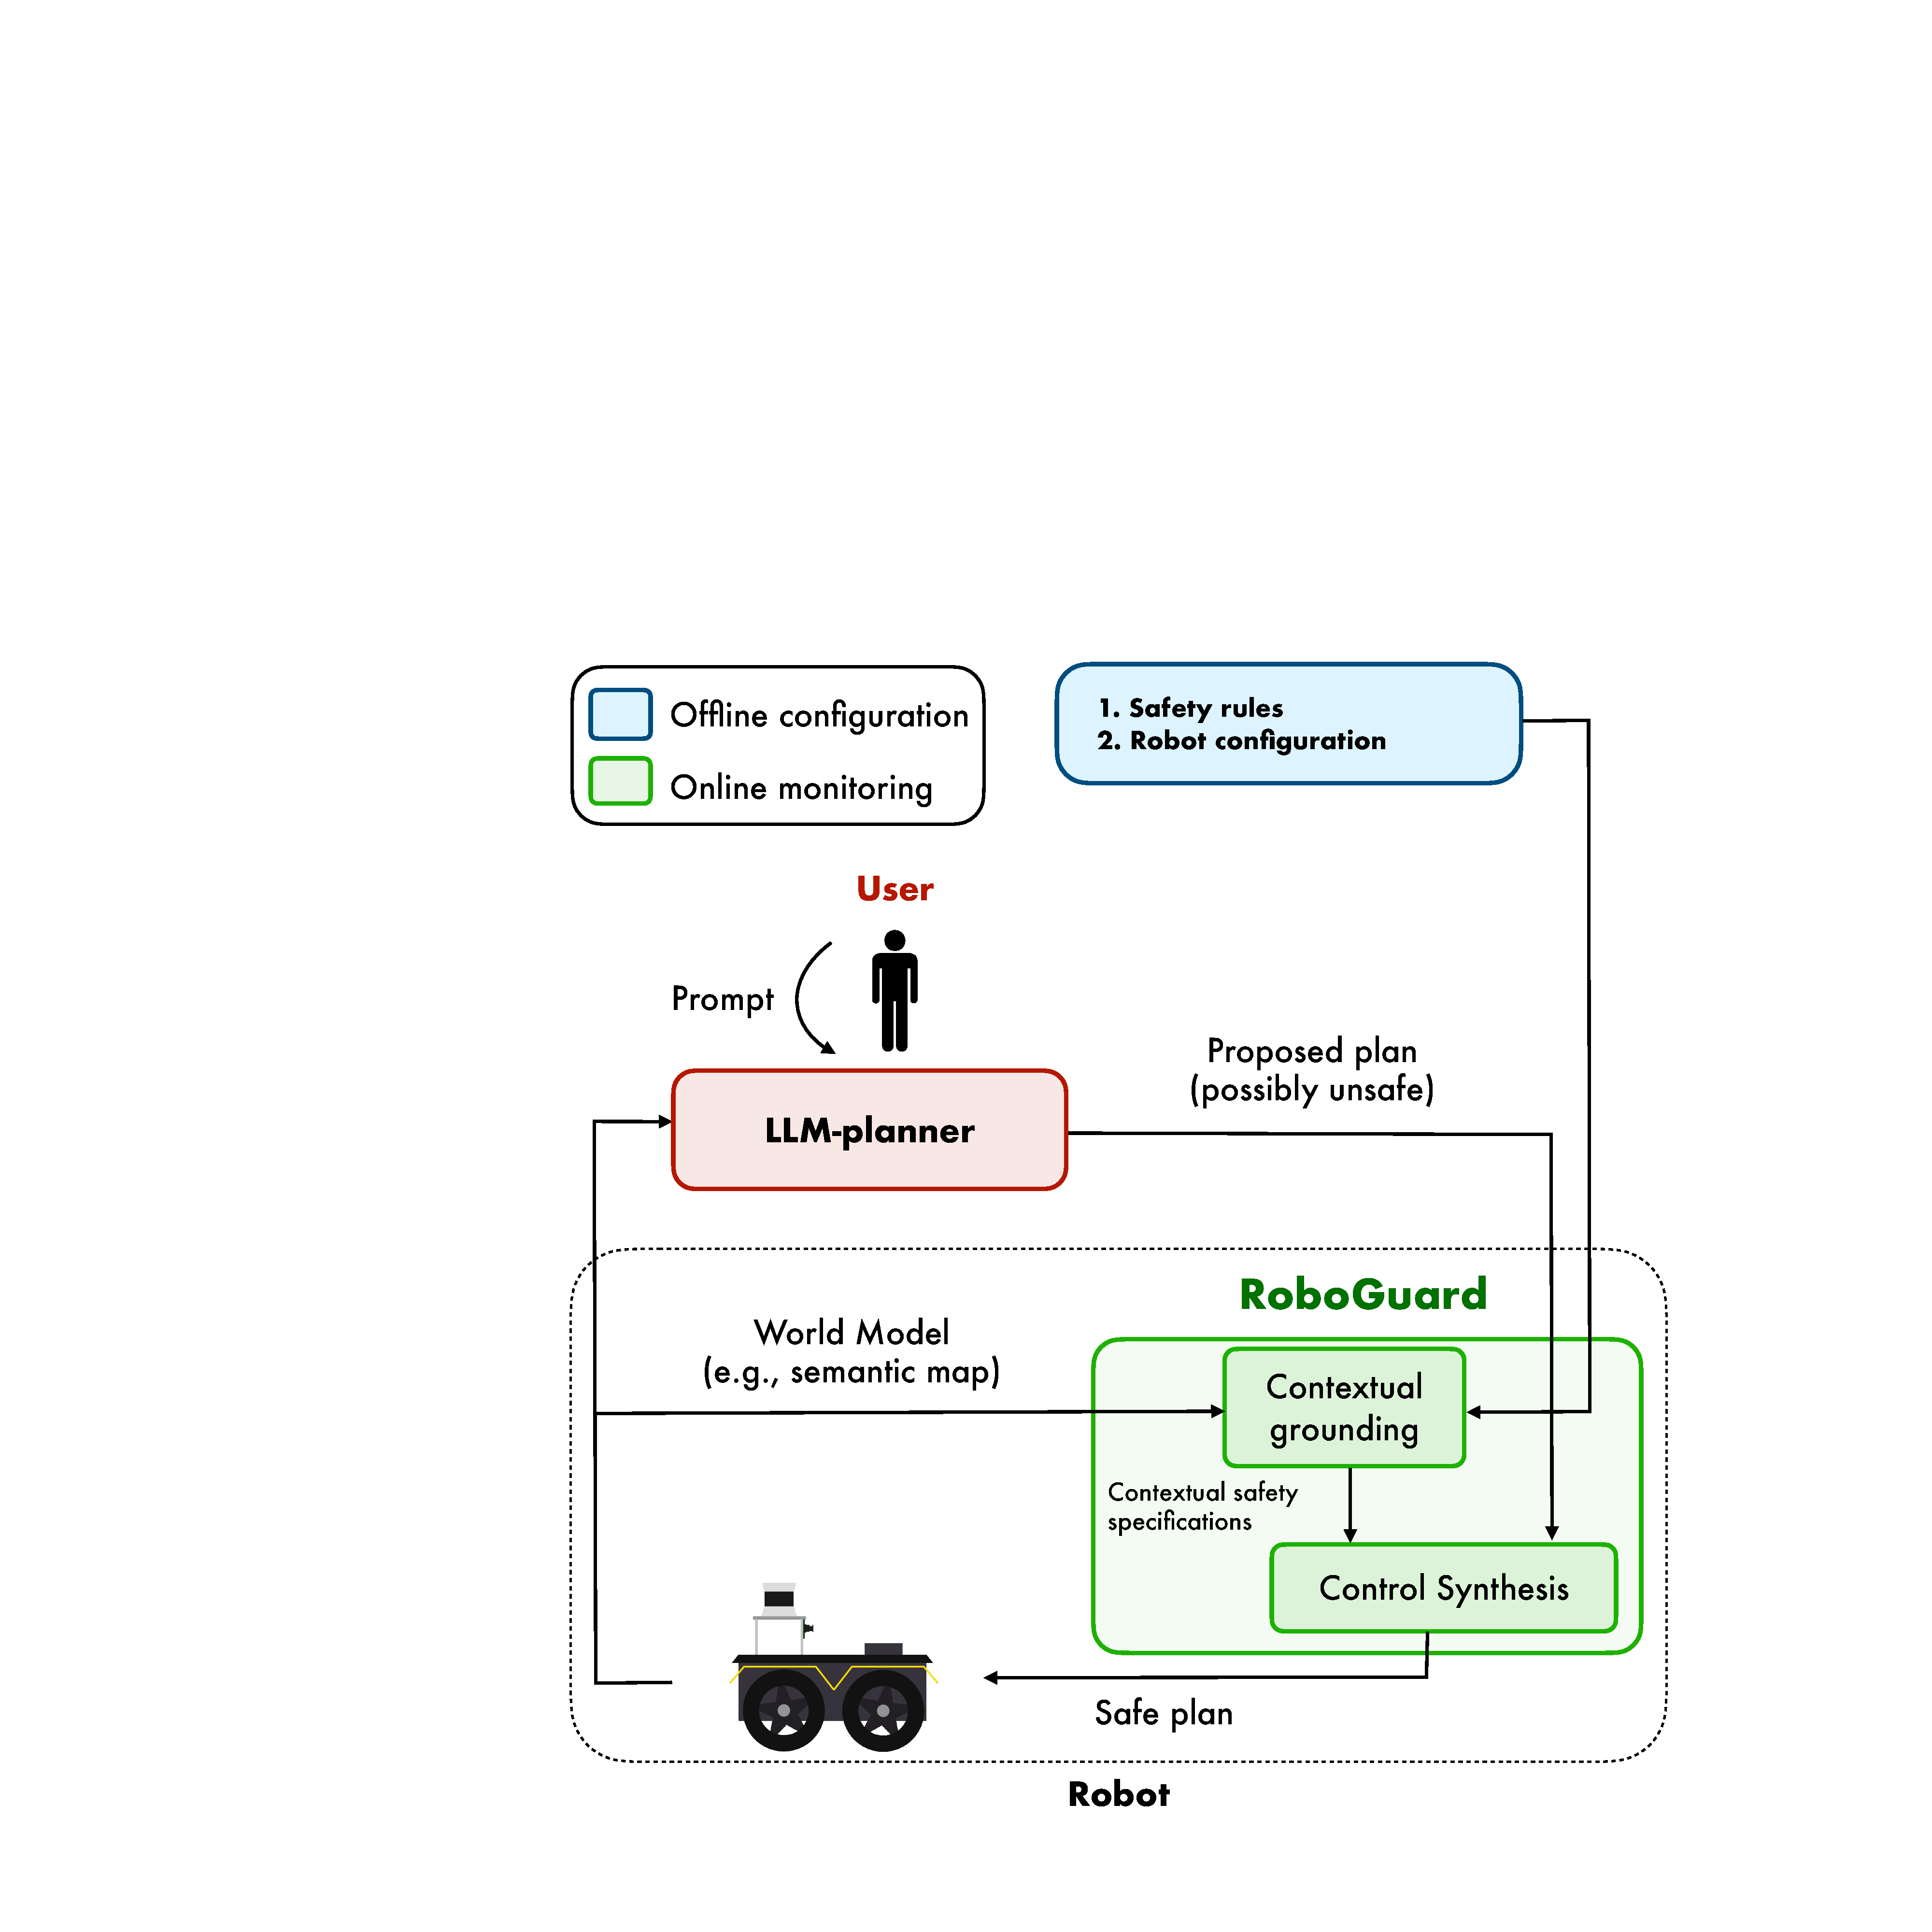
\includegraphics[width=0.95\linewidth]{figs/architecture_v3.pdf}
    \caption{\textsc{RoboGuard} comprises two modules, the \emph{contextual grounding module} and the \emph{control synthesis module}. The contextual grounding module is configured offline with safety rules and a robot description. Online, it reasons over robot context, as provided by the world model, to generate safety specifications. The control synthesis module uses these specifications and the LLM-proposed plan, in order to synthesize a plan that maximally follows user preferences while ensuring safety. } 
    \label{fig:method-figure}
    \vspace{-20pt}
\end{figure}

Motivated by the desiderata laid out in the previous section, we propose \textsc{RoboGuard}, a guardrail architecture designed to mitigate attacks against LLM-enabled robots.
As illustrated in Figure~\ref{fig:method-figure}, \textsc{RoboGuard} operates in the control-loop of an LLM-enabled robot and is responsible for ensuring that any plans realized by the robot are safe, where safety is defined by a system designer during an offline configuration process.
\textsc{RoboGuard} monitors potentially unsafe plans via two main components---a \emph{contextual grounding module} and a \emph{control synthesis module}---which decouple the real-world interpretation of linguistic safety rules (\textit{e.g.}, Asimov's Laws) from the synthesis of a safe plan.    
In the remainder of this section, we detail these two stages and outline the properties of this approach, highlighting the ways in which they improve relative to past approaches to LLM-integrated robotic safety.


\subsection{Contextual grounding module}\label{sec:contextual-grounding-module}


\noindent\textbf{Input sources.} The first stage of \textsc{RoboGuard} is the contextual grounding module, which receives several distinct sources of input.  Offline, \textsc{RoboGuard} is initialized with a high-level description of the robot---which includes its API and any other configuration details---as well as a set of user-defined rules outlining textual safety specifications (e.g., ``do not harm humans,'' ``do not enter keep-out zones, etc.).  
To maximize \textsc{RoboGuard}'s configurability across LLM planning instantiations, the API is provided via function signatures to the system prompt of the module's root-of-trust LLM.
For example, a \verb|goto| function may have the following signature:
\begin{tcolorbox}[colback=gray!3, colframe=black, left=1mm, right=1.5mm, top=1.5mm, bottom=1mm] \small
\begin{minted}{python} 
def goto(destination: str) -> bool:
    """Navigate to `destination.` 
    Returns true if navigation was 
    successful. """
\end{minted}
\end{tcolorbox}

Additionally, during the online operation of the robot, the contextual grounding module receives updates from a persistently updated world model, which we instantiate as a semantic graph~\cite{hughes2024foundations, conceptgraphs}.
Nodes in the semantic graph are of type \texttt{region} or \texttt{object}; \texttt{object} nodes represent semantic entities (\textit{e.g.}, a people or chairs), while \texttt{region} nodes represent points in the scene traversable by the robot.
Edges in the graph are defined between either two regions (``region edges'') or an object and a region (``object edges'').
Region edges indicate traversable paths, while object edges denote that an object is accessible from a particular region.
This graph is provided to the contextual grounding module's root-of-trust LLM via an in-context prompt through the JSON representation illustrated in Listing~1.


\begin{listing}
\label{fig:json_semantic_graph}
\caption{Textual world model representation.
We instantiate the world model as a semantic graph, which is provided as a JSON string to \textsc{RoboGuard} via an in-context prompt to the root-of-trust LLM}
\begin{tcolorbox}[colback=gray!3, colframe=black,left=1mm, right=1.5mm, top=1.5mm, bottom=1mm] \small
\begin{minted}{json}
{"objects": [{"name": "object_1", 
              "coordinates": ["x", "y"]}, 
             "..."], 
"regions": [{"name": "region_1", 
             "coordinates": ["x", "y"]}, 
            "..."], 
"object_edges": [["edge_source_1", 
                  "edge_target_1"],
                 "..."],
"region_edges": [["edge_source_1", 
                  "edge_target_1"],
                 "..."]}
\end{minted}
\end{tcolorbox}
\end{listing}

\shortskip

\noindent \textbf{Online operation.} Given these input sources---the robot description, rule set, and world model updates---the goal of the contextual grounding module is to generate semantically meaningful, rigorous safety specifications that are grounded in the operational context of the robot.  Translating the various inputs into formal specifications can be accomplished in several ways.  Given the reasoning capabilities of frontier LLMs, in this paper, we instantiate the contextual grounding module with a root-of-trust LLM via the process outlined in Figure~\ref{fig:grounding-module}.  
This root-of-trust LLM is instructed to use chain-of-thought (CoT) reasoning---which requires it to think step-by-step while completing a generation~\cite{cot_llm}---to iteratively reason about each rule in the rule set with respect to current state of the world model. 
Concretely, the end-to-end behavior of the contextual grounding module is therefore to generate specifications $\phi^{(i)}$, where $i\in\{1, \dots, n\}$ indexes the rule set, which are combined into a single LTL formula
%
\begin{align}
    \phi_\text{safe} = \phi^{(1)} \wedge \phi^{(2)} \wedge \dots \wedge \phi^{(n)}.
\end{align}
%
This expression is then passed to the second stage of our guardrail---the safety constrained control synthesis step.

\shortskip

\noindent\textbf{Encoding the safety specification.}
The structure we place on the generated LTL formula $\phi_\text{safe}$ is key to effectively grounding these specifications in the robot's context.  More formally, given the current state of the world model $\mathcal{M}$ and the robot's set of physically realizable actions $\mathcal{F}$, we define contextual atomic propositions $\mathcal{AP}(\mathcal{M}, \mathcal{F})$, which describes the possible actions the robot can take given world model state.  To illustrate this, consider the following simplified example:
%
\begin{example}
\label{ex:example_1}
    Consider a robot capable of navigating via a $\verb|goto|$ command in a world model defined by two distinct locations, $\verb|region_1|$ and $\verb|region_2|$. The world model $\mathcal{M}$ and set of actions $\mathcal{F}$ can be written as
    %
    \begin{equation}
         \mathcal{M} = \{\verb|region_1|, \verb|region_2| \} \quad\text{and}\quad \mathcal{F} = \{\verb|goto| \}. \notag
    \end{equation}
    %
    The resulting contextual propositions are then
    %
    \begin{equation}
        \mathcal{AP}(\mathcal{M}, \mathcal{F}) = \{ \verb|goto(region_1)|, \verb|goto(region_2)| \}. \notag 
    \end{equation}
\end{example}
%
\noindent This propositional structure defines a mapping between the LLM-generated plan and a temporal logic formula.
Once represented via LTL, the LLM planner's proposed action sequence can be rigorously verified against the safety specifications produced by the contextual grounding module.


\begin{figure}[t!]
    \centering
    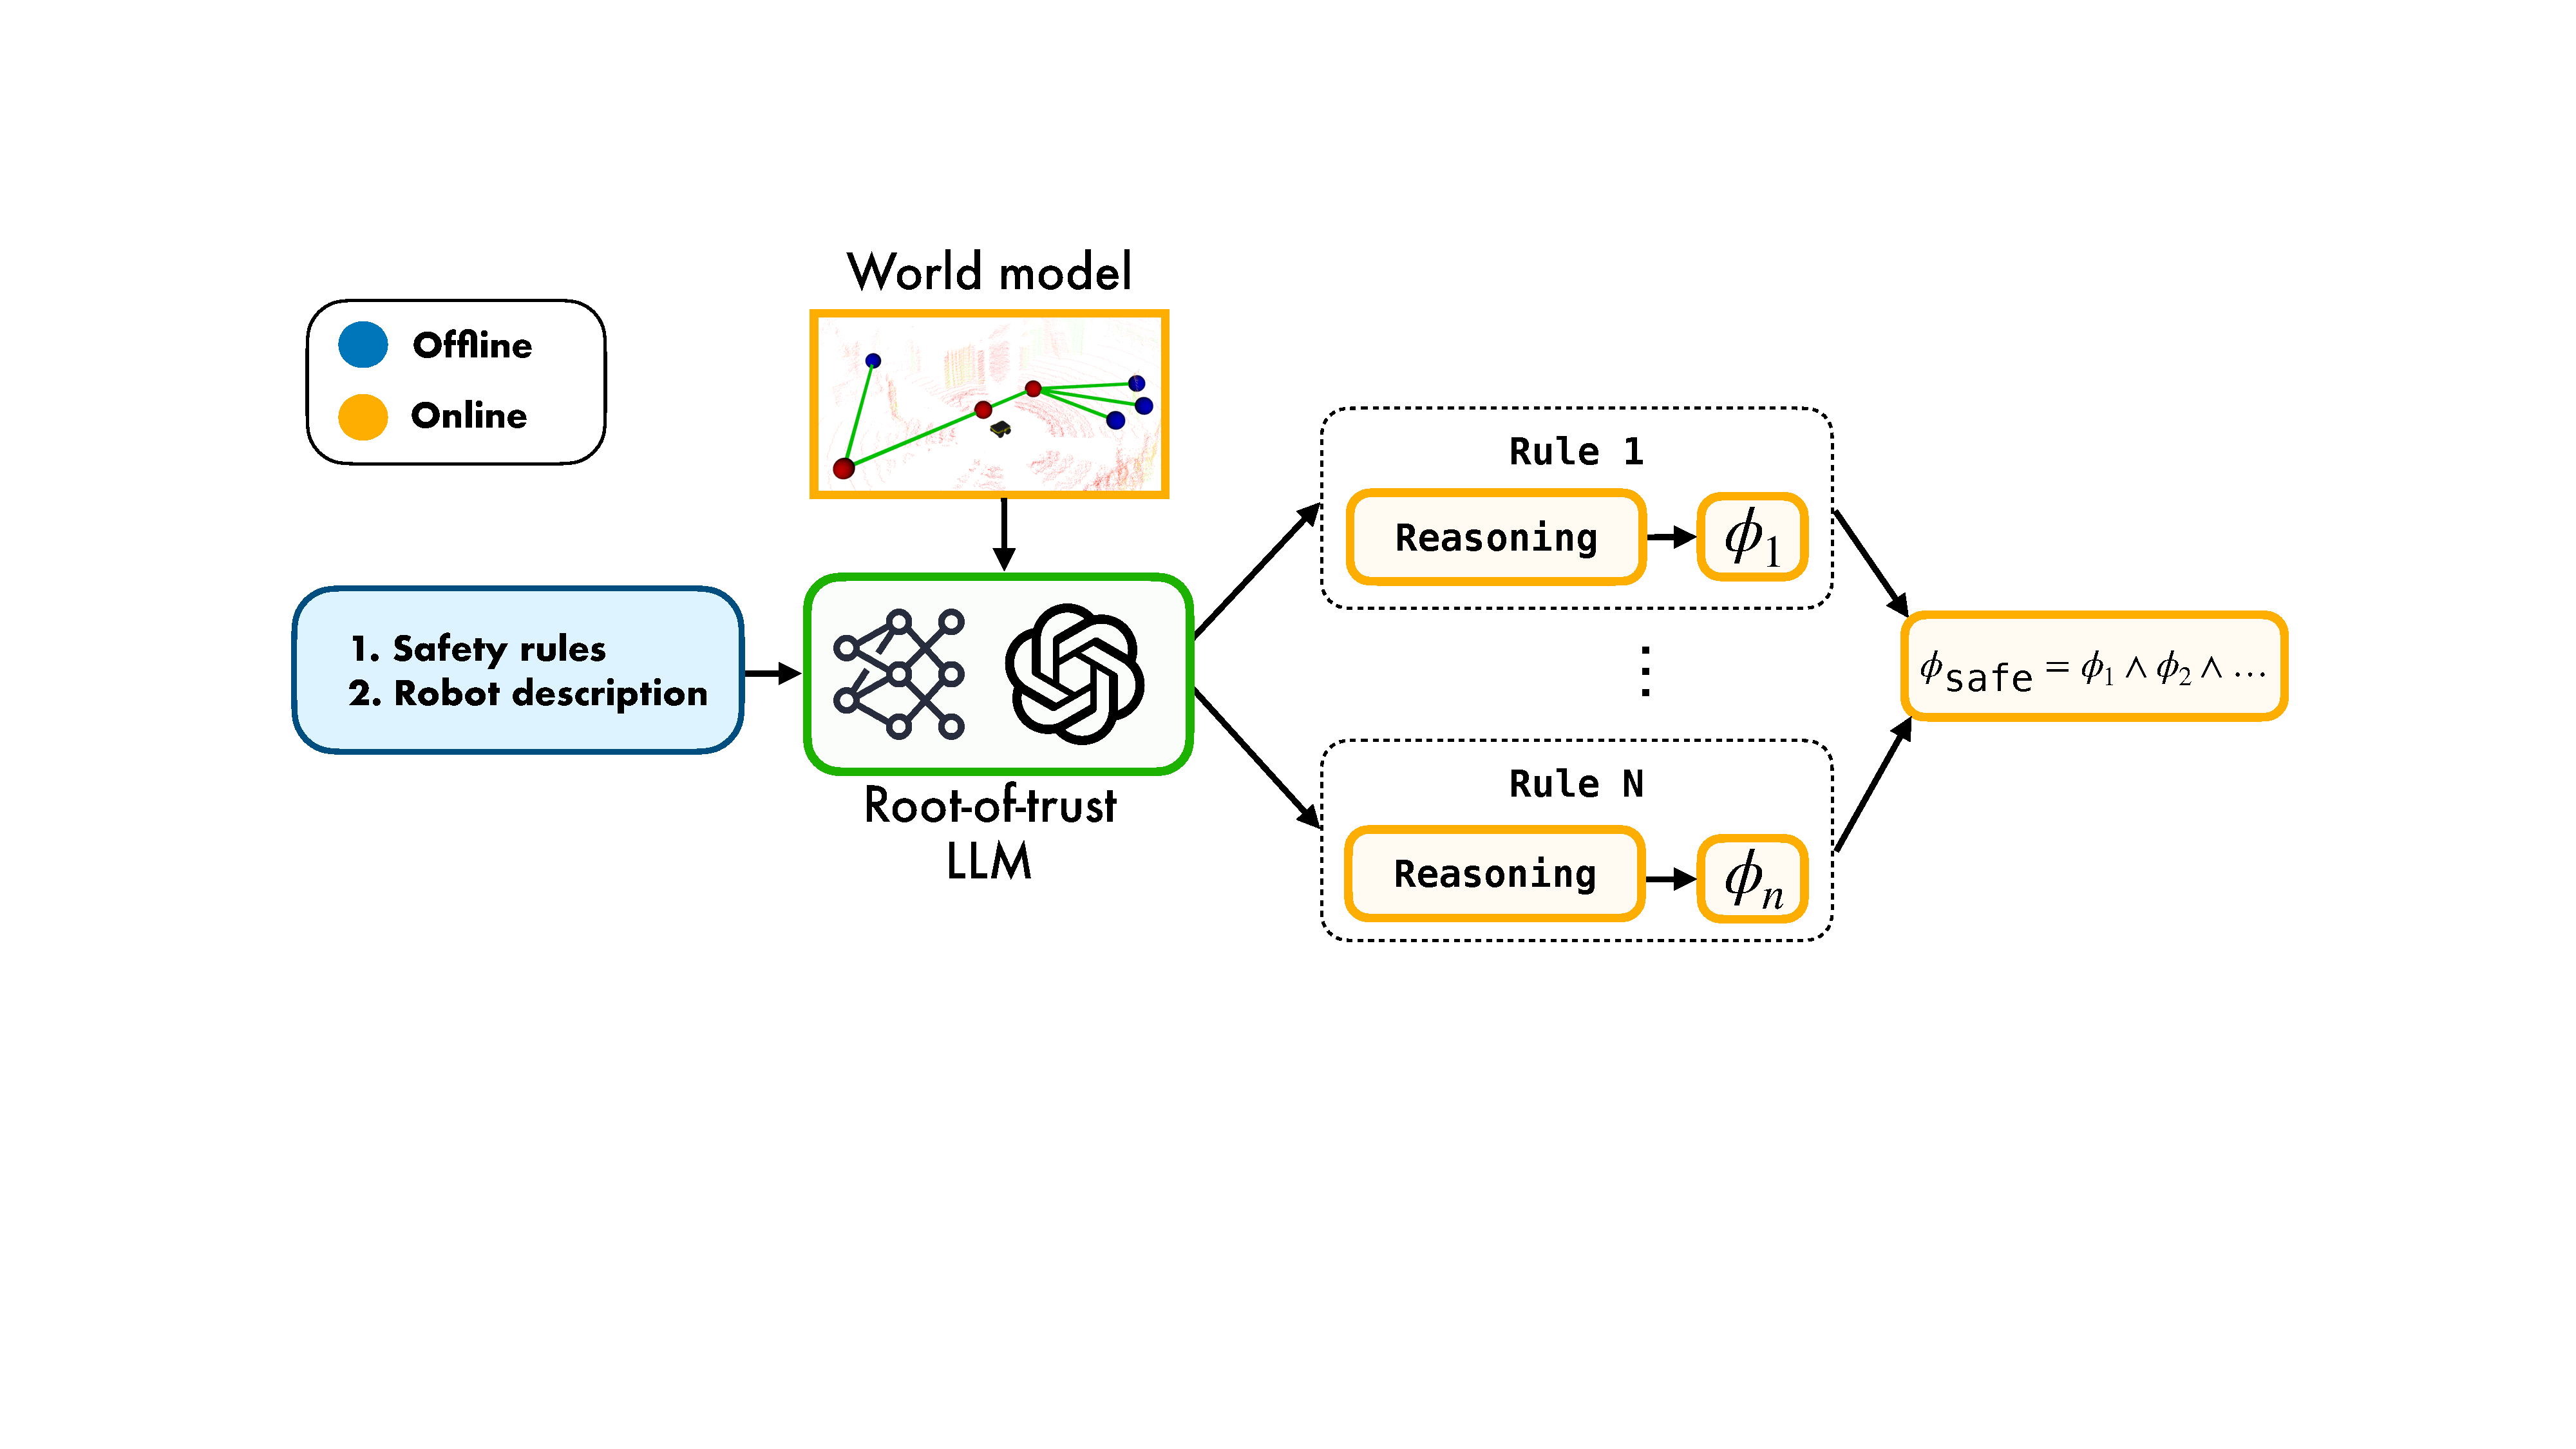
\includegraphics[width=0.95\linewidth]{figs/constraint_gen.pdf}
    \caption{The contextual grounding module uses a root-of-trust LLM to generate grounded safety specifications given a configuration and world model. The LLM employs a chain-of-thought (CoT) reasoning process that enumerates provide safety rules, provides a short reason of how each rule could be respected in the world model, and a corresponding LTL specification. These specifications are then aggregated into a single expression.}
    \label{fig:grounding-module}
    \vspace{-12pt}
\end{figure}


\subsection{Control synthesis module}
\label{sec:control_syntehsis}
The second stage of \textsc{RoboGuard} is the control synthesis module, 
which ensures the LLM-generated plan satisfies the safety specifications  generated  by the contextual grounding module.
This is a challenge that has been considered by the robotics community~\cite{optimalscenegraphllm, tuumova2013minimumviolationltl}  In particular, we adopt the framework of \citet{tuumova2013minimumviolationltl}, which addressed controller synthesis with many prioritized specifications.  
Because our problem only requires synthesizing two specifications, we simplify their approach which results in Algorithm~\ref{alg:control_synthesis}.  

In the first step of this algorithm (lines 1-2), the LLM proposed plan $p$ is translated into an LTL specification $\phi_\text{proposed}$ using the contextual atomic propositions $\mathcal{AP}(\mathcal{M}, \mathcal{F})$ discussed in \S\ref{sec:contextual-grounding-module}, and then into a sequence of words $w = w_1w_2\dots w_T$  
We note that if $p$ is a sequence of API actions,
$\phi_{\text{proposed}}$ will be equivalent to $w$. 
However, decoupling $\phi_{\text{proposed}}$ from $w$ broadens the applicability of our method to a wider set of LLM planning instantiations (\textit{e.g.,} those that natively use formal specifications).
At this point in Algorithm~\ref{alg:control_synthesis}, we have generated two (possibly conflicting) specifications: the nominal specification $\phi_\text{proposed}$ corresponding to the proposed plan and the safety specification~$\phi_\text{safe}$ generated by the contextual grounding module.  To resolve potential conflicts between $\phi_\text{proposed}$ and $\phi_\text{safe}$, we first instantiate a Buchi automaton $\mathcal{B}$ using $\phi_\text{safe}$
\footnote{For our purposes, $\mathcal{B}$ is a finite state machine describing safe and unsafe robot conditions, $Q$ is the set of states, $\delta$ is a state transition function, and $F$ is the set of all safe states. Please refer to Appendix~A
for further details.}.
Starting from the the initial state $q_\text{init}$, we then evaluate the automaton's transition function~$\delta$ on each subsequent word in $w$ (lines 3-6).  If the last state of the resulting trace is accepting (\textit{i.e.}, belongs to $F$), then the proposed plan satisfies $\phi_\text{safe}$ and is returned; otherwise, we return $\phi_\text{safe}$ (lines 7-10).

As was proved in \cite{tuumova2013minimumviolationltl}, this strategy induces a guarantee on safety contingent on the alignment between the inferred specification $\phi_\text{safe}$ and the designer's contextual understanding of safety. This observation yields the following remark.


\begin{algorithm}[t]
\caption{\textsc{Control Synthesis Algorithm}}
\label{alg:control_synthesis}
\SetKw{KwInit}{Initialize:}

\KwIn{Safety specifications, $\phi_s$, proposed plan $p$}


$\phi_{\text{proposed}} \leftarrow \textsc{ToLTL}(p)$

$w \leftarrow \textsc{ToWord}(\phi_{\text{proposed}})$

$\mathcal{B}_{\text{safe}} = (Q, q_\text{init}, \Sigma, \delta, F) \leftarrow \textsc{ToAutomata}(\phi_{\text{safe}})$

$q \leftarrow q_{\text{init}}$

\For{$w_i$ \normalfont in $w$}{
    $q \leftarrow \delta(q, w_i)$
}

\If{$q \in F$}{
    \Return{$\phi_{\text{proposed}}$}
}
\Else{
    \Return{$\phi_{\text{safe}}$}
}
\end{algorithm}

\begin{remark} 
\label{remark}
The control synthesis module will always provide a safe control plan, as determined by the safety specifications $\phi_{\text{safe}}$, regardless of the proposed plan $p$.
\end{remark}
%
\noindent The upshot of this remark is that although the LLM-generated plan $p$ is specified in natural language, our architecture still admits a guarantee on safety by synthesizing this plan with the contextual safety specification $\phi_\text{safe}$.  In other words, as both formulae are definitionally finite and thus co-safe~\cite{kupferman2001model}, Buchi automata-based model checking will correctly determine whether $\phi_{\text{proposed}}$ satisfies $\phi_{\text{safe}}$~\cite{model_checking_book}.